
\documentclass[procedia]{easychair}
\usepackage[utf8]{inputenc}
\usepackage{cite}
\usepackage{algorithmic}
\usepackage{array}
\usepackage{hyperref}
\usepackage{url}
\usepackage{mathtools}
\hyphenation{op-tical net-works semi-conduc-tor method methods}
\usepackage{float}
\usepackage[font=scriptsize]{subcaption}
\usepackage[font=scriptsize]{caption}

\DeclareGraphicsExtensions{.pdf,.jpeg,.jpg,.png}

\floatstyle{ruled}
\newfloat{json}{thp}{lop}
\floatname{program}{Program}

\institute{Neter, Finland}

\title{A Simulator for Event-oriented Data in Flexible Assembly System Fault Prediction – PRE-PRINT}
\titlerunning{A Simulator for Event-oriented Data in Flexible Assembly System Fault Prediction – PRE-PRINT}
\author{Tero Keski-Valkama}
\authorrunning{Tero Keski-Valkama}

\begin{document}

\maketitle

\keywords{Discrete Event Simulation, Flexible Assembly System, Anomaly Detection}

\begin{abstract}
We present an open source discrete event simulator, FAS Simulator, for generating interleaved process traces of Flexible Assembly Systems. The simulation includes plausible faults creating anomalies in the output.
The generated outputs can be used as a benchmark for evaluating novel anomaly detection methods.
\end{abstract}

\section{Introduction}
This paper describes a method for simulating event-oriented data sources of a flexible assembly system (FAS) including faults. Such a simulator is required for creating representative corpuses
of data for teaching automated learning algorithms for predictive maintenance, condition monitoring and systemic fault detection.

Flexible assembly system was described by Donath and Graves \cite{donath1988flexible} as a collection of flexible assembly cells comprising one or several work stations connected by automatic material-handling devices.
In practise, a flexible assembly system contains parts and materials stored in an intermediate storage,
a conveyor or crane system to move the parts, materials, intermediate assemblies and finished products between the stations, and the stations with work machines and necessary tooling
to assemble, process or inspect intermediate assemblies and products. The stations might consist of for example manual assembly steps, and robotic assembly cells. In flexible manufacturing systems (FMS),
the work stations might contain more complex machining and manufacturing tools like CNC lathes, or 3D printing. FAS and FMS are considered interchangeable for the purposes of this article, although
they have different scheduling and configuration properties.
Often the assembly sequence has multiple ways of being executed for a finished product leading to some redundancy and more efficient scheduling in terms of utilization.

As opposed to more specialized industrial production systems, flexible assembly systems are designed for smaller batches and greater flexibility so that the set of end products can vary more widely.
Flexible assembly systems can be reconfigured more conveniently following the evolution of new versions of the end products. Flexibly assembly systems also allow for a wider range
of customization between the different end product instances of the same product. The nature of fast evolution of configurations and workflows, and varying operating conditions make
planning maintenance more challenging.

System downtime is a significant cost for flexible assembly systems. System downtime is reduced by preventive maintenance typically scheduled periodically.
Recently Internet of Things and opening of the networked industrial system APIs have created new possibilities for predictive maintenance and systemic fault detection. Different sites with similar
flexible automation systems have widely different environmental and workload conditions which has an impact on the wear and tear of the flexible automation system components.
There is a clear need to adapt maintenance based on actual conditions in the operation rather than by simply scheduling maintenance periodically\cite{hashemian2011state}.

Going from preventive maintenance towards predictive maintenance optimizes and targets the maintenance related costs towards the activities that have best impact
on improving the availability and operation of deployed flexible assembly systems.

Predictive maintenance in flexible assembly systems benefits from automatic indicators for immediate and potential future faults.
It is generally not possible to enumerate all the possible fault conditions and their sensory indicators of a flexible assembly system in an exhaustive fashion,
as the rare errors are neglected and faults can present in an unexpected manner\cite{camarinha1996integration}.
There is a need for autonomously learning systems which are able to deduce the correct operation of the flexible assembly system and report potential deviances. One way to monitor a process is to observe the symbolic
logs generated as the process is being executed.

Current predictive maintenance and condition monitoring systems concentrate on measuring device health for example by means of measuring temperature\cite{mobley2002introduction},
vibration\cite{scheffer2004practical}, lube oil particle analysis\cite{hunt1993handbook} and electrical current signals
\cite{thomson2001current}. Research on anomaly detection for non-interleaved discrete sequences is summarized in a survey by Varun Chandola et al.\cite{chandola2012anomaly}
Interleaved discrete sequences, or uncorrelated process traces have been mainly researched in relation to specification mining for multi-threaded or asynchronous software processes.
A solution for mining message sequence graphs by Sandeep Kumar et al.\cite{kumar2011mining} works for message-oriented systems,
and this solution requires sets of separate and complete traces corresponding to executions of an application\cite{mining-program-workflow-from-interleaved-traces}.

In process mining there are several approaches in automatically extracting process models such as Alpha algorithm and its 
variants, genetic process mining, heuristic process mining, multi phase mining, and region-based process mining. In general these algorithms work with log messages labelled with the process instance.

Some success have been reported by Niels Landwehr using Mixture Hidden Markov Models \cite{landwehr2008modeling} in labelling interleaved activities from event logs.
However, these methods require manual labelling of the training data and are therefore unsuitable for an unsupervised setting.
A method used in parallel software workflow mining described here \cite{mining-program-workflow-from-interleaved-traces} requires the execution logs to be separated into
a large number of complete runs, and would not work with a flexible assembly system in a continuous operation.

Most process mining and specification mining
solutions aim to solve the challenging task of inferring a complete process model out of the logs, even if the interleaved logs themselves might exhibit some weaker form of features
and characteristics already useful for anomaly detection.

Evaluating novel automatic methods for fault prediction requires standard benchmarks to compare these methods against. Currently there are no standard benchmarks to test
different symbolic log anomaly detection methods and compare their performance against each other. Realistic and plausible simulations are often used\cite{jager2014assessing}\cite{FASTTRIPS} for domains where
real data is hard to collect or where real data would be subject to business confidentiality. Training neural networks and other learning systems often utilizes realistic
simulations instead of real data\cite{weston2014memory}. Real measured data is often limited in both state space and in volume,
and simulations can give better results \cite{duch2005artificial}.

Some simulations of flexible assembly systems are generally available\cite{giulio}\cite{el1989simulation}\cite{donath1988flexible} and have been studied for visualization and optimization purposes.
However, these are not directly suitable for benchmarking fault detection methods regarding interleaved process traces.

\section{Problem Formulation}

Real data regarding flexible assembly system faults is
not generally available, because fault data is generally subject to business confidentiality in flexible assembly industry.
The generally available simulation models do not contain failure modes and are not designed to emit
log structured events in a realistic fashion.

To enable relevant research into anomaly detection in flexible assembly systems a realistic simulator for logged events is needed.
All references to simulated faults and failure modes in the research described in this article are hypothetical and should not be considered to
reflect actual characteristics of any specific existing systems. An effort is made to make the simulations contain the necessary features of
generic and realistic failure modes to make the models useful for research, but for example the simulated fault frequencies and the configuration
of the flexible assembly system along with workflows and end products are arbitrary.

A simulation for benchmarking anomaly and fault detection methods should not be fully deterministic to reflect the real world dynamics. The simulation should also
include realistic faults with possible early indicators such as variations in delays in the steps of the process. The focus of the simulator is on faults without pre-existing
diagnostic fault codes, such as unexpected faults, degradation of the assembly modules and conveyors, and on systemic faults. Systemic faults in this paper
are defined to mean faults and degradation of output where each of the component modules of the flexible assembly system are seemingly operating without faults. Execution failures
which are detected during execution of an action as a deviance of the state from the expected state are outside of the focus of this work, as these conditions are adequately detected and handled
by existing supervision systems.

Ultimately, the learning system should model the correct operation of the system and detect deviances, rather than to learn specific failure modes which might never repeat after presenting once.

Flexible assembly system process traces are not separable into complete and separate execution runs in the general case, because assembly process is typically continuous and
forms a single interleaved log.
On the other hand, delays in processing steps are mostly independent of the whole system state, and could be hypothetically used to infer structure in the interleaved log.
There are also events unrelated to the processes, for example timer ticks. The main process events often follow stoichiometric laws in a normal operation corresponding to materials
not being created or destroyed within the process. Stoichiometric invariance is often clearly visible when drawing a histogram of event type counts in the logs showing that specific events corresponding to certain
assembly steps are done specific numbers of times per product, leading to counts of events for a specific event type strongly correlating with counts of other event types.

\section{Modes of Failures in Flexible Assembly Systems}

Flexible assembly system failures are typically component failures where a failure of a single module or a component will lead to the part of the system becoming inoperational.
Since the flexible assembly systems are dynamic systems with numerous moving parts, the wear and tear of the components and tools are a significant source of faults.

In addition to the component failures, certain critical systemic failures can cause downtime, such as power loss and network communication failures.
The critical systemic failures mentioned don't typically show any indication before they happen so predictive maintenance has little potential to be applied there.
In addition to these critical system failures,
the whole system can exhibit modes of failure and degradation which are not directly attributable to single component degradation or failure.
Some of these might be caused by
external factors, such as accidents and human errors, but also for example by timing issues in the whole process causing unexpected queues or traffic jams.

Tool wear and tear depends on the workload. Typically tools that wear out fast, for example multiple times for one unit of work in a station, receive much attention and such tools are generally
well maintained. Tools that have wear and tear but have longer life spans are more susceptible to being overlooked by operators and might have some indicators of degrading
before a failure. Cranes, hatches and conveyors have relatively long life spans and are primarily maintained in periodic preventive maintenance. If we could get indicators
for impending failure for these components, the periodical maintenance could be scheduled earlier to prevent downtime.

In addition to these physical faults the flexible
assembly system can suffer from human errors. Human operator can inadvertently misconfigure the flexible assembly system so that its operating mode changes unexpectedly,
for example by disabling a station which can lead to the system stopping without a proper failure. In addition to configuration
errors, human operators might fail in manual assembly steps for example by pressing the button to mark the step
as completed before the step was completed.
The flexible assembly system might also get in incompatible materials, parts or replacement tools and fail when trying to use them.

There has lately been an increase of computer crime against industrial networks as the devices and systems become more connected.
Nation states execute industrial espionage and even sabotage against each other\cite{stuxnet}. An electronic sabotage attack might present itself
much like a human misconfiguration error, and would be potentially detected in a similar fashion even if the attack itself would not be
directly visible in the logs to intrusion detection systems.

For the purposes of describing the fault types we divide system components into slowly and
quickly degrading tools and auxilliary components. Tools are the components such as drill bits which are directly used to assemble or
machine the product. The auxilliary components are components with less expected wear and tear which are used to transport the products,
inspect the intermediate assemblies or dispense assembly components.

\begin{table}[bt]
\tiny
\renewcommand{\arraystretch}{1.3}
\caption{Table of recognized fault types in flexible assembly systems}
\label{faults}
\centering
\begin{tabular}{|p{50mm}|p{25mm}|p{25mm}|p{25mm}|}
\hline
Fault type & Unexpected faults & Potentially has an early indication & Useful target for anomaly detection \\
\hline
\hline
Auxilliary component wear and tear & X & X & X \\
\hline
Station operation failures (feeder error, insertion error, grip error, fixture position errors) & & & \\
\hline
Critical systemic failures (power, network, emergency stop) & X & & \\
\hline
Human error, failed manual step & X & X & X \\
\hline
Incompatible parts, materials or replacement tools & X & & \\
\hline
Systemic failures (e.g. accidents and cyberattacks) & X & X & X \\
\hline
Tool wear and tear for quickly degrading tools (e.g. drill bits) & & X & \\
\hline
Tool wear and tear for slowly degrading tools (e.g. screwdriver) & X & X & X \\
\hline
\end{tabular}
\end{table}

The fault types and distribution depend on the assembly system
and on the products being assembled. For one
specific assembly line \cite{cong1997fault} the common fault types were feeder errors, robot insertion errors,
robot grip errors, unqualified parts, fixture position errors, emergency stops, robot gripper collision,
grip sensor line break, and inspection equipment failures. The root causes for these are wear and tear, and incompatible parts.

For useful anomaly detection systems we need to concentrate on faults that are unexpected without pre-existing diagnostic error codes, and that potentially have early indications
in collected event-based logs. Early indication in this context means that the error can be detected in the system logs before the failure becomes otherwise evident.
The Table \ref{faults} summarizes the classes of faults and their respective potential for anomaly detection.

\section{Flexible Assembly System Model}

The simulation consists of a realistic discrete event model of a flexible assembly system with faults optionally injected into the process.
The initial simulation is very simple and linear, and does not incorporate complex scheduling and routing decisions or optimization like many flexible assembly/manufacturing system simulations\cite{donath1988flexible}.
However, it is a reasonable configuration of such a production system. Introducing synthetic faults into process data is a common method for testing whether the fault detection model works \cite{able2016model}.

FAS processes are often modelled as colored Petri nets \cite{saitou2002robust}, where a colored token corresponds to each process instance, moving between process states at observed events.
In the scope of this research the process instances are not known, and all events are interleaved together for each process instance running concurrently. In the absence of distinction between process instances
and by extension the Petri net tokens, the most appropriate formal model is a Petri Net.

Discrete Event Systems can be conveniently
described using Mixed Process Algebra Petri Nets (MPPN)\cite{falkman2001modeling}. In the following description we augment the MPPN with intervals between state transitions,
because event intervals are important information for deinterleaving the process traces.

Using the notation defined in \cite{falkman2001combined}, we note that the system can be described as an interleaved execution of $ n $ process instances $ P_i $, shown in
Equation \ref{interleaved_processes}.
\begin{equation}
 P_1 \oplus P_2 \oplus ... \oplus P_n
 \label{interleaved_processes}
\end{equation}

The interleaved process instances consist of sequences of $ m $ steps which are identical within a production batch in the simple assembly process being tested, shown in Equation \ref{identical_steps}.
More complex assembly processes might have several alternatives for specific steps, representing multiple interchangeable stations where an unit of work can be scheduled.
It is also possible for some processes that some assembly steps can be performed in an arbitrary order.
The sets B and U above the arrows denote the booking/unbooking sets constraining this transition, encapsulating the scheduling dependencies between process instances.
\begin{equation}
 P_i = a_1 \xrightarrow{B_2 \& U_1} a_2 \rightarrow ... \rightarrow a_m
 \label{identical_steps}
\end{equation}

Some steps are associated with exclusive resources which can be described by associating the transitions in the MPPN model with booking and unbooking resources, so that
the corresponding transitions $ b_l(x) $ and $ u_l(x) $ for a single resource $ R_l $ in the general resource model Petri net shown in \ref{resource_model} trigger changes in the status of the resource and
are gated by the status of the resource.

\begin{equation}
 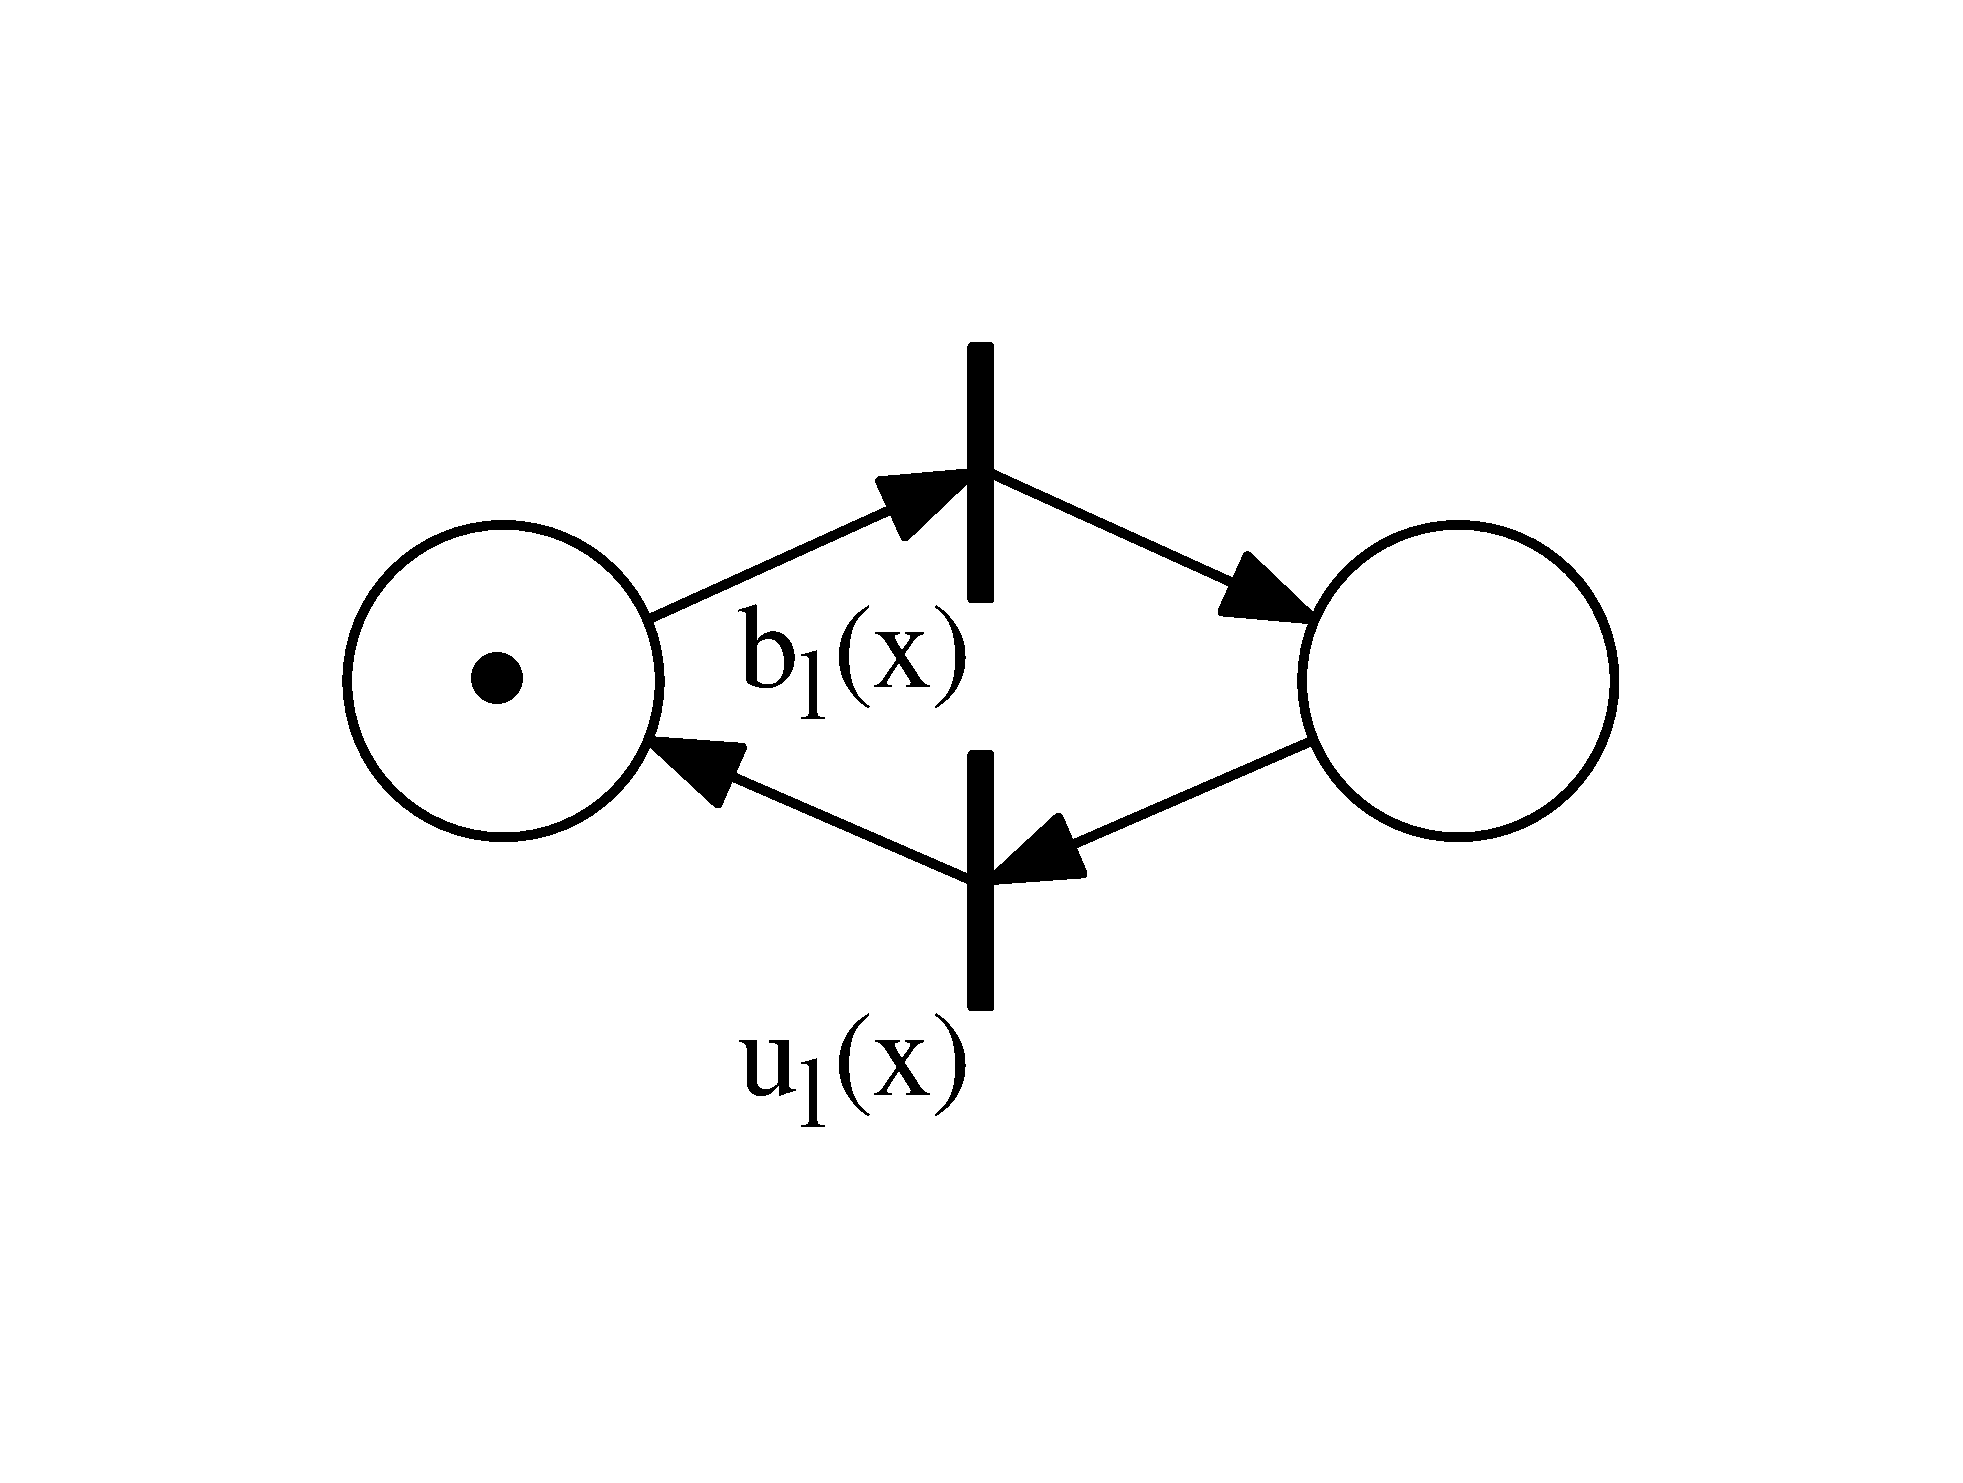
\includegraphics[width=4 cm,keepaspectratio=true]{./general_resource_model.eps}
 \label{resource_model}
\end{equation}

The logs generated by the FAS Simulator can be described as a set of sequences each describing a successful assembly of one product instance shuffled, or interleaved
together.
A formal language that accepts such sequences is called a shuffled language \cite{berglund2011recognizing}. These languages are context-sensitive, so modelling methods
relating to regular and context-free languages are inadequate. For example Langer et al. \cite{langer2011self} showed that Angluin learner was able to learn small
toy examples very well, but didn't work very well for a real world example of a stream of events recorded from a CAN bus of the powertrain network of an electric vehicle.

The simulator is implemented in Python using Simpy discrete event simulation framework and it generates a JSON file which models the logs from the system.
The log messages consist of a timestamp and an event type.

The discrete event simulation framework consists of a scheduler that takes the next event from the event queue and applies it to the respective module. The simulated modules
execute when events are applied to them, and generate new events and immediate log entries with timestamps.
The simulated modules have optional failure modes that affect the simulated operation of the component. Failure modes are configured to the simulated modules
by scheduling failure activation as separate unlogged events.
The main executable sets up the configuration of the processes, and bootstraps the events and optional faults.

The simulated hypothetical system assembles and tools a car transmission block loosely inspired by a Youtube video of Chrysler transmission assembly\cite{transmission}.
The linear workflow consists of several manual assembly steps in separate stations and transporting the subassemblies between the stations by the means of
cranes and conveyors. Multiple transmission blocks in different stages of assembly are being assembled simultaneously in different stations.

The main sequence starts from the frame of the transmission block
and continues through several manual steps done in separate stations. The steps of the main sequence are given in the software documentation\cite{FASSimulator}.
Each step contains several events and associated log messages.
The non-negative durations follow a truncated normal distribution. The durations for manual steps in normal operation have a standard deviation of five percent of the mean. The durations for automatic steps
have a standard deviation of one percent of the mean.

\subsection{Simulated Failure Modes}
It is regrettable that real data on fault modes in real flexible assembly systems is not publicly available. It is still possible to make reasonable
models based on existing data from other analogous sources such as \cite{nasaames} and \cite{tsarouhas2009classification}. In FAS Simulator, the fault modes
can be reasonably expected to reflect the real conditions. Initially, we will simulate two types of wear and tear delays.

Generally mechanical wear and tear effect on machine health profile follows
an accelerating curve downwards \cite{eker2012major}, \cite{milldataset}. For the purposes of simulation we can assume machine health has an approximately
linear effect on machine performance measured in delays and success rates in applicable types of faults.

Simulated wear and tear causes two types of delay profiles.
First, a continuous wear and tear typically causes no measurable delays at first, but when the degradation accumulates the delay increases following
a roughly exponential curve shown in the Figure \ref{figure:continuouswearandtear}.

Second, for certain steps, such as taking bolts from the bowl feeder a human operator
might fail to grab a bolt from time to time. Typically the human operator tries again until successful. The frequency of the failure increases
slowly and roughly following an exponential curve. This characteristic delay profile is depicted in the Figure \ref{figure:retrydelays}.

\begin{figure}[tb]
\tiny
\begin{subfigure}[h]{0.47\linewidth}
 \resizebox{\linewidth}{!}{% Title: glps_renderer figure
% Creator: GL2PS 1.3.9, (C) 1999-2015 C. Geuzaine
% For: Octave
% CreationDate: Fri Jul 28 20:08:47 2017
\setlength{\unitlength}{1pt}
\begin{picture}(0,0)
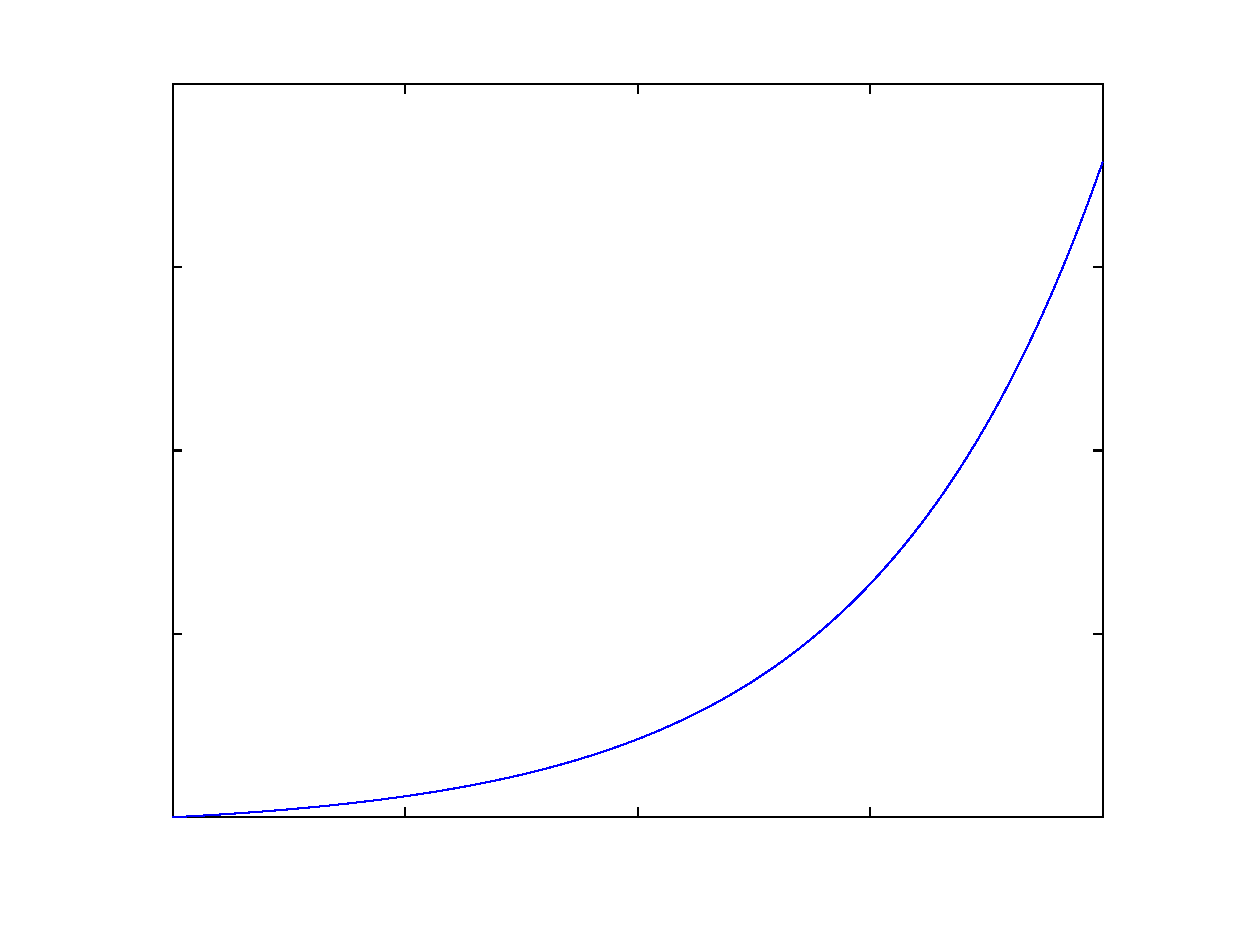
\includegraphics{failure_profile-inc}
\end{picture}%
\begin{picture}(576,433)(0,0)
\fontsize{10}{0}
\selectfont\put(74.8799,43.519){\makebox(0,0)[t]{\textcolor[rgb]{0,0,0}{{0}}}}
\fontsize{10}{0}
\selectfont\put(186.48,43.519){\makebox(0,0)[t]{\textcolor[rgb]{0,0,0}{{5}}}}
\fontsize{10}{0}
\selectfont\put(298.08,43.519){\makebox(0,0)[t]{\textcolor[rgb]{0,0,0}{{10}}}}
\fontsize{10}{0}
\selectfont\put(409.68,43.519){\makebox(0,0)[t]{\textcolor[rgb]{0,0,0}{{15}}}}
\fontsize{10}{0}
\selectfont\put(521.28,43.519){\makebox(0,0)[t]{\textcolor[rgb]{0,0,0}{{20}}}}
\fontsize{10}{0}
\selectfont\put(69.8755,48.52){\makebox(0,0)[r]{\textcolor[rgb]{0,0,0}{{1}}}}
\fontsize{10}{0}
\selectfont\put(69.8755,136.54){\makebox(0,0)[r]{\textcolor[rgb]{0,0,0}{{1.5}}}}
\fontsize{10}{0}
\selectfont\put(69.8755,224.56){\makebox(0,0)[r]{\textcolor[rgb]{0,0,0}{{2}}}}
\fontsize{10}{0}
\selectfont\put(69.8755,312.58){\makebox(0,0)[r]{\textcolor[rgb]{0,0,0}{{2.5}}}}
\fontsize{10}{0}
\selectfont\put(69.8755,400.6){\makebox(0,0)[r]{\textcolor[rgb]{0,0,0}{{3}}}}
\fontsize{10}{0}
\selectfont\put(298.08,32.519){\makebox(0,0)[t]{\textcolor[rgb]{0,0,0}{{time index t (fault at index 0)}}}}
\fontsize{10}{0}
\selectfont\put(50.8755,224.56){\rotatebox{90}{\makebox(0,0)[b]{\textcolor[rgb]{0,0,0}{{delay factor}}}}}
\fontsize{10}{0}
\selectfont\put(298.08,410.6){\makebox(0,0)[b]{\textcolor[rgb]{0,0,0}{{(exp(t / 5.0) - 1) / 30 + 1}}}}
\end{picture}
}
 \caption{A delay profile of continuous wear and tear\newline}
 \label{figure:continuouswearandtear}
\end{subfigure}
\begin{subfigure}[h]{0.47\linewidth}
 \resizebox{\linewidth}{!}{% Title: glps_renderer figure
% Creator: GL2PS 1.3.9, (C) 1999-2015 C. Geuzaine
% For: Octave
% CreationDate: Fri Jul 28 20:08:48 2017
\setlength{\unitlength}{1pt}
\begin{picture}(0,0)
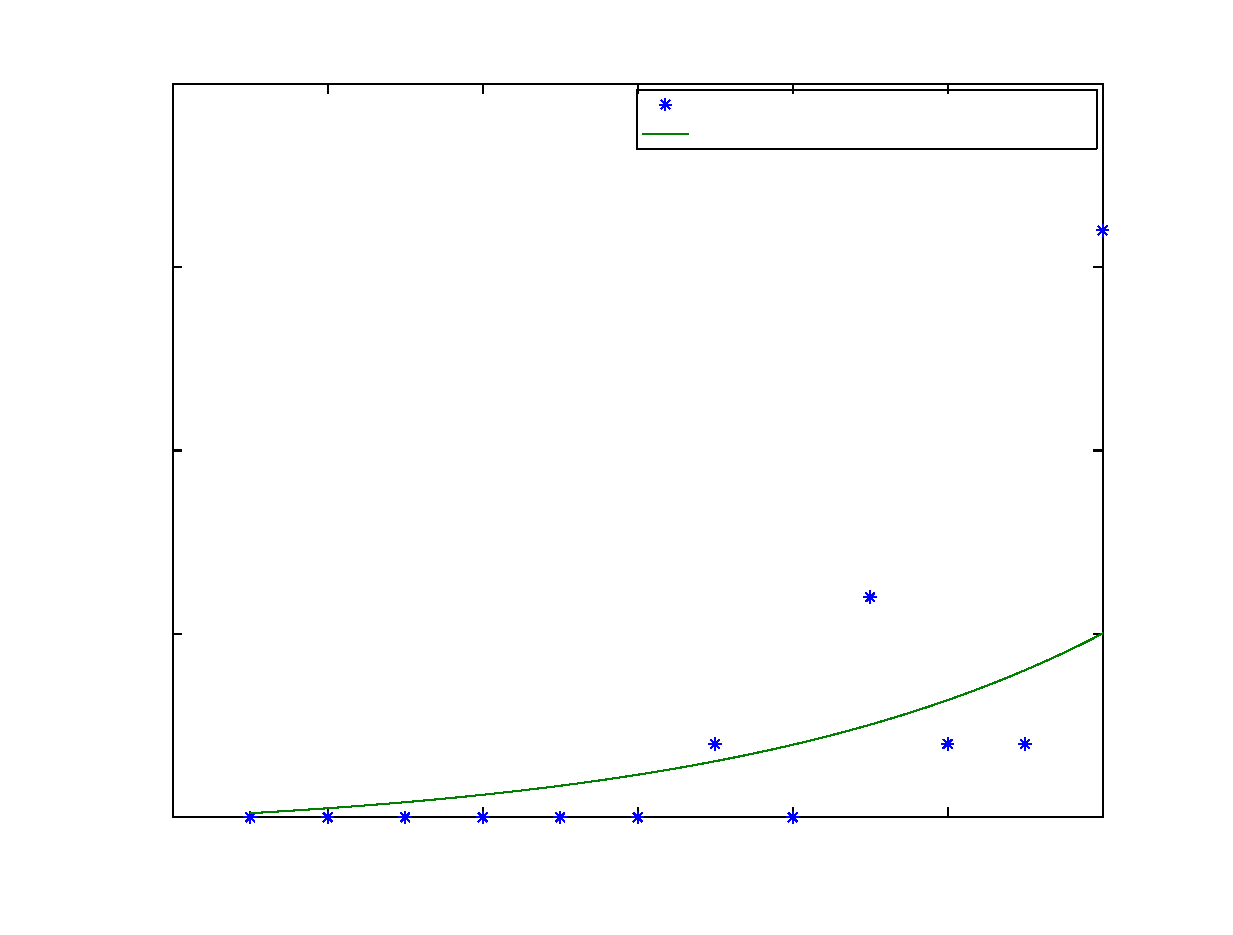
\includegraphics{retry_profile-inc}
\end{picture}%
\begin{picture}(576,433)(0,0)
\fontsize{10}{0}
\selectfont\put(74.8799,43.519){\makebox(0,0)[t]{\textcolor[rgb]{0,0,0}{{0}}}}
\fontsize{10}{0}
\selectfont\put(149.28,43.519){\makebox(0,0)[t]{\textcolor[rgb]{0,0,0}{{2}}}}
\fontsize{10}{0}
\selectfont\put(223.68,43.519){\makebox(0,0)[t]{\textcolor[rgb]{0,0,0}{{4}}}}
\fontsize{10}{0}
\selectfont\put(298.08,43.519){\makebox(0,0)[t]{\textcolor[rgb]{0,0,0}{{6}}}}
\fontsize{10}{0}
\selectfont\put(372.48,43.519){\makebox(0,0)[t]{\textcolor[rgb]{0,0,0}{{8}}}}
\fontsize{10}{0}
\selectfont\put(446.88,43.519){\makebox(0,0)[t]{\textcolor[rgb]{0,0,0}{{10}}}}
\fontsize{10}{0}
\selectfont\put(521.28,43.519){\makebox(0,0)[t]{\textcolor[rgb]{0,0,0}{{12}}}}
\fontsize{10}{0}
\selectfont\put(69.8755,48.52){\makebox(0,0)[r]{\textcolor[rgb]{0,0,0}{{1}}}}
\fontsize{10}{0}
\selectfont\put(69.8755,136.54){\makebox(0,0)[r]{\textcolor[rgb]{0,0,0}{{1.5}}}}
\fontsize{10}{0}
\selectfont\put(69.8755,224.56){\makebox(0,0)[r]{\textcolor[rgb]{0,0,0}{{2}}}}
\fontsize{10}{0}
\selectfont\put(69.8755,312.58){\makebox(0,0)[r]{\textcolor[rgb]{0,0,0}{{2.5}}}}
\fontsize{10}{0}
\selectfont\put(69.8755,400.6){\makebox(0,0)[r]{\textcolor[rgb]{0,0,0}{{3}}}}
\fontsize{10}{0}
\selectfont\put(298.08,32.519){\makebox(0,0)[t]{\textcolor[rgb]{0,0,0}{{time index t (fault at index 0)}}}}
\fontsize{10}{0}
\selectfont\put(50.8755,224.56){\rotatebox{90}{\makebox(0,0)[b]{\textcolor[rgb]{0,0,0}{{delay factor}}}}}
\fontsize{10}{0}
\selectfont\put(325.188,390.612){\makebox(0,0)[l]{\textcolor[rgb]{0,0,0}{{Sampled random delays from Poisson}}}}
\fontsize{10}{0}
\selectfont\put(325.188,376.429){\makebox(0,0)[l]{\textcolor[rgb]{0,0,0}{{Mean delay profile}}}}
\fontsize{10}{0}
\selectfont\put(298.08,410.6){\makebox(0,0)[b]{\textcolor[rgb]{0,0,0}{{poissrnd((exp(t / 5.0) - 1) / 4) * 0.2 + 1}}}}
\end{picture}
}
 \caption{A characteristic delay profile of human operator retry delays}
 \label{figure:retrydelays}
\end{subfigure}
 \caption{Delay profiles of faults.}
 \label{figure:delayprofiles}
\end{figure}

The simulated failures and their effects are listed in the Table \ref{failures}. To have a meaningful simulation of a system under faults we only need to simulate some representative fault conditions.

\begin{table}[tb]
\tiny
\renewcommand{\arraystretch}{1.3}
\caption{Table of the simulated failures}
\label{failures}
\centering
\begin{tabular}{|p{40mm}|p{40mm}|p{50mm}|}
\hline
Failure & Description & Effect \\
\hline
\hline
Failed manual step & The human operator tries again until successful & A poisson distribution of delay for the step 7 \\
\hline
Wear \& tear & The completion time for the step degrades & The delay for the step 20 is exponential \\
\hline
\end{tabular}
\end{table}

\section{Implementation}

The FAS Simulator\cite{FASSimulator} is implemented in Python as a discrete event simulator using Simpy discrete event simulation library.
Each step of the assembly process is a Simpy resource and a process which receives and generates
delayed events in model time. Each step of the assembly process manages its own internal state, and possible failure modes.

The example simulation consists of stereotypical models of the steps of the process. For example, simulating
the operation of a crane an instance of a module named Crane is configured and added to the respective position in the process in relation to other module instances.
The Crane module has a capacity of one item to transport at a time, and generates delayed output events for each of the input event in sequence, so that only one item is
transported at a time. This is in contrast to conveyor module instances which don't have a limited capacity, as the conveyors transport the items independently and in parallel.

The simulation is set up by first defining the all the modules in the assembly plant. The actual simulation
is done simply by triggering the global process inputs as required, causing sequences of events being generated accordingly. For interleaved process traces we instantiate multiple
parallel processes that share the resources in the simulated assembly plant.

Several specific simulation runs are pre-defined for the purposes of benchmarking
different modelling approaches.
Each type of simulation can also be configured to fail in specific ways to test different failure detection approaches.

In addition to the events related to specific process traces, there is an event for an alarm if the queue waiting for a manual process is larger than five items. Also, there is
a periodical ``tick'' event for every 10 seconds. One conveyor is reused for two process steps, the steps 6 and 9. This means that these conveyor events
trigger twice for each product.

Three different simulation runs of around 1400 events and 36 event types are shown in Figure \ref{figure:output_images}. Figure \ref{figure:output_easy} shows a normal, fault-free production run.
The run consists of 30 items assembled simultaneously, going through the system.
The pixel colors correspond to event types. The end is padded with gray.

\begin{figure}[b]
\begin{subfigure}[h]{0.32\linewidth}
 \resizebox{\linewidth}{!}{\input{./output_easy.tex}}
 \caption{A normal run without faults.\newline\newline}
 \label{figure:output_easy}
\end{subfigure}
\begin{subfigure}[h]{0.32\linewidth}
 \resizebox{\linewidth}{!}{\input{./output_easy_with_wear_and_tear_fault.tex}}
 \caption{The same as previous, but with a simulated wear and tear fault in the step 15 conveyor.}
 \label{figure:output_easy_wear_and_tear}
\end{subfigure}
\begin{subfigure}[h]{0.32\linewidth}
 \resizebox{\linewidth}{!}{% Title: glps_renderer figure
% Creator: GL2PS 1.3.9, (C) 1999-2015 C. Geuzaine
% For: Octave
% CreationDate: Sat Jul 29 15:05:29 2017
\setlength{\unitlength}{1pt}
\begin{picture}(0,0)

\includegraphics{output_easy_with_retry_delay_fault-inc}
\end{picture}%
\begin{picture}(576,433)(0,0)
\fontsize{10}{0}
\selectfont\put(180.9,43.519){\makebox(0,0)[t]{\textcolor[rgb]{0,0,0}{{10}}}}
\fontsize{10}{0}
\selectfont\put(292.5,43.519){\makebox(0,0)[t]{\textcolor[rgb]{0,0,0}{{20}}}}
\fontsize{10}{0}
\selectfont\put(404.1,43.519){\makebox(0,0)[t]{\textcolor[rgb]{0,0,0}{{30}}}}
\fontsize{10}{0}
\selectfont\put(515.7,43.519){\makebox(0,0)[t]{\textcolor[rgb]{0,0,0}{{40}}}}
\fontsize{10}{0}
\selectfont\put(69.8755,355.333){\makebox(0,0)[r]{\textcolor[rgb]{0,0,0}{{5}}}}
\fontsize{10}{0}
\selectfont\put(69.8755,305.036){\makebox(0,0)[r]{\textcolor[rgb]{0,0,0}{{10}}}}
\fontsize{10}{0}
\selectfont\put(69.8755,254.738){\makebox(0,0)[r]{\textcolor[rgb]{0,0,0}{{15}}}}
\fontsize{10}{0}
\selectfont\put(69.8755,204.441){\makebox(0,0)[r]{\textcolor[rgb]{0,0,0}{{20}}}}
\fontsize{10}{0}
\selectfont\put(69.8755,154.144){\makebox(0,0)[r]{\textcolor[rgb]{0,0,0}{{25}}}}
\fontsize{10}{0}
\selectfont\put(69.8755,103.847){\makebox(0,0)[r]{\textcolor[rgb]{0,0,0}{{30}}}}
\fontsize{10}{0}
\selectfont\put(69.8755,53.5498){\makebox(0,0)[r]{\textcolor[rgb]{0,0,0}{{35}}}}
\end{picture}
}
 \caption{The same as Figure \ref{figure:output_easy}, but with a simulated retry delay fault in the step 7 bowl feeder.}
 \label{figure:output_easy_retry_delay}
\end{subfigure}
 \caption{The event sequences as colored pixels from left to right, top to bottom, padded in the end with gray.}
 \label{figure:output_images}
\end{figure}

For comparison, Figure \ref{figure:output_easy_wear_and_tear} was
created for situation where a simulated wear and tear fault happens in one of the conveyors, slowing its operation down slightly. Comparing the two simulations visually it is evident that the second process
is slower in the end of the batch, featuring tick events in longer sequences.
Similarly a retry delay fault with the bowl feeder can be seen in the Figure \ref{figure:output_easy_retry_delay}. As the retry delay affects a process step that is relatively fast, and does not 
represent a bottleneck in the process, it does not have a significant impact to the total process time. However, a learning algorithm could in principle notice variations of delays between specific events
and flag an anomaly.

\section{Conclusion}

This study presents a benchmark model for validating anomaly detection methods for flexible assembly systems using log structured data.
Existing systems for predictive maintenance concentrate on measuring health of separate devices based on typical degradation characteristics
for such devices. They also concentrate on continuous measurement data instead of symbolic log entries. In process mining the methods assume the process instances are identified.

The diagnostic data for flexible assembly systems is a closely guarded secret for business reasons, but it is possible to make reasonable models
of faults based on other analogous sources.

The Flexible Assembly System Simulator, FAS Simulator, is published in GitHub \cite{FASSimulator} as open source. While the simulation
approach adds an indirection between real data and developed methods, it is necessary to veil the business critical real fault and diagnostic
data of the flexible assembly systems but still make the different anomaly detection methods comparable. The simulator also provides means to incorporate new types of
failures and test anomaly detection methods in a quick iteration.

Additional research is needed to improve this benchmark simulation by using experiences from real flexible assembly systems and their modes of failure
and respective future fault indicators.

\label{sect:bib}
\bibliographystyle{plain}
\bibliography{FAS-Simulator_YSC2017_Tero_Keski-Valkama_easychair_procedia}

\appendix

\end{document}
